\documentclass[footline=authortitle]{beamer}
\usepackage{graphicx} % Required for inserting images
\usepackage[dvipsnames]{xcolor}
\usepackage[english]{babel}
\usepackage{ragged2e}
\usepackage{hyphenat}
\usepackage{siunitx}

\usepackage{listings}
\usepackage{xcolor}
\usepackage{wrapfig}


\lstset{
  language=Python,
  basicstyle=\ttfamily\footnotesize,
  keywordstyle=\color{blue},
  commentstyle=\color{gray},
  stringstyle=\color{orange},
  showstringspaces=false,
  breaklines=true,
}

\usepackage{biblatex}
\nocite{*}
\addbibresource{bib.bib}

\mode<presentation>{
  \usetheme{Frankfurt}
  \usecolortheme[named=PineGreen]{structure}
  \useoutertheme{default} % solo UNA volta
  \setbeamertemplate{headline}{}  % rimuove del tutto la barra in alto

  \makeatletter
  \setbeamertemplate{footline}{
    \leavevmode%
    \hbox{%
      \begin{beamercolorbox}[wd=.65\paperwidth,ht=2.5ex,dp=1ex,center]{author in head/foot}%
        \usebeamerfont{author in head/foot}\insertshortauthor
      \end{beamercolorbox}%
      \begin{beamercolorbox}[wd=.1\paperwidth,ht=2.5ex,dp=1ex,center]{frame number in head/foot}%
        \insertframenumber{} / \inserttotalframenumber
      \end{beamercolorbox}%
      \begin{beamercolorbox}[wd=.25\paperwidth,ht=2.5ex,dp=1ex,center]{title in head/foot}%
        \usebeamerfont{title in head/foot}\insertshorttitle
      \end{beamercolorbox}%
    }
    \vskip0pt%
  }

  \setbeamercovered{transparent}
  \setbeamercolor{block title example}{fg=white,bg=Blue}
  \setbeamercolor{block body example}{fg=black,bg=Blue!10}
  \setbeamercolor{postit}{fg=black,bg=OliveGreen!20}
  \setbeamercolor{postit2}{fg=yellow,bg=OliveGreen}
}

\title[Computational Imaging]{Meteorological Super-Resolution\\vs\\Wind Representations}
\author[Gruppo 21 - Marzia De Maina, Matteo Galiazzo, Federica Santisi]
{Gruppo 21\\Marzia De Maina, Matteo Galiazzo, Federica Santisi}
\institute[Alma Mater Studiorum - Università di Bologna]
{
  \textit{Alma Mater Studiorum - Università di Bologna}\\[0.25Cm]
  \textit{Dipartimento di Informatica - Scienza e Ingegneria (DISI)} \\[0.5Cm]
  
  }
\date{}
\begin{document}
\begin{frame}[fragile]
    \titlepage
    
\end{frame}

\begin{frame}{Purpose}
  \begin{itemize}
  \justifying
    \item[-] Evaluate the impact of \textbf{different wind representations} on neural-based super-resolution for meteorological fields.
    \vspace{0.2cm}
    \item[-] Compare two \textbf{wind encodings}:
      \begin{itemize}
        \item[-] Orthogonal components $u_{10},\,v_{10}$
        \item[-] Polar form: speed and direction (degrees from north)
      \end{itemize}
    \vspace{0.2cm}
    \item[-] Use \textbf{ERA5} (\textit{30 km}) and \textbf{VHR-REA} (\textit{2.2 km}) datasets for training and testing.
    \vspace{0.2cm}
    \item[-] Assess which representation yields better performance and qualitative reconstruction.
  \end{itemize}
\end{frame}

% MARZIA
% Wind Field Representations
\begin{frame}{Wind Field Representations}
      \textbf{Cartesian Components}\
      \begin{itemize}
        \item[-] $u_{10}, v_{10}$: zonal and meridional wind at 10m height
        \item[-] Directly match ERA5 outputs
      \end{itemize}
      \vspace{0.5cm}
      \textbf{Polar Encoding}\
      \begin{itemize}
        \item[-] $\text{speed}=\sqrt{u_{10}^2 + v_{10}^2}$
        \item[-] $\text{direction}=(180 + \frac{180}{\pi}\arctan2(-u_{10}, -v_{10}))\bmod360$
      \end{itemize}
  \vspace{0.5cm}
  \textbf{Motivation:} Representation may affect neural network learning and reconstruction quality.
\end{frame}
% riprendere la consegna ricordando che consegna avevamo, cosa era richiesto e fare una panoramica sulla teoria necessaria (unet)

%%%%% Super-Resolution
\begin{frame}{Super-Resolution}
\textbf{Super-Resolution}\\\justifying
Upscaling low-resolution fields to high-resolution targets using deep learning. This tecnique involves reconstructing high-resolution images from coarser data, with the aim of capturing finer and more complex atmospheric structures.
\begin{figure}
    \centering
    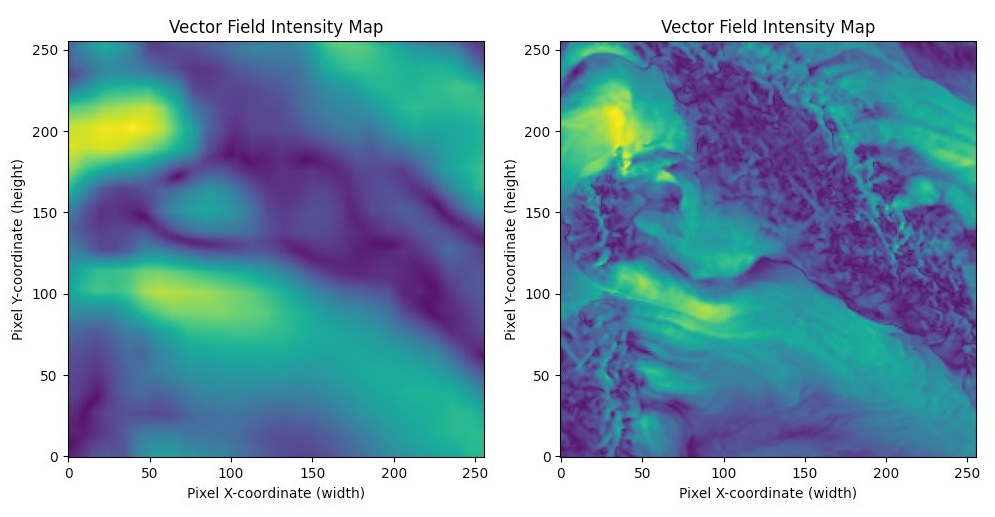
\includegraphics[width=0.8\linewidth]{images/img_superris.jpeg}
    \caption{Super-resolution in the best case}
    \label{fig:enter-label}
\end{figure}
\end{frame}

%%%%% U-Net Theory
\begin{frame}{U-Net}
    \textbf{U-Net Architecture}\\Encoder-decoder with skip connections for image-to-image tasks.
      \begin{itemize}
        \item[-] Residual blocks to ease training.
        \item[-] Multiscale features preserved via concatenation.
      \end{itemize}
      \begin{figure}
          \centering
          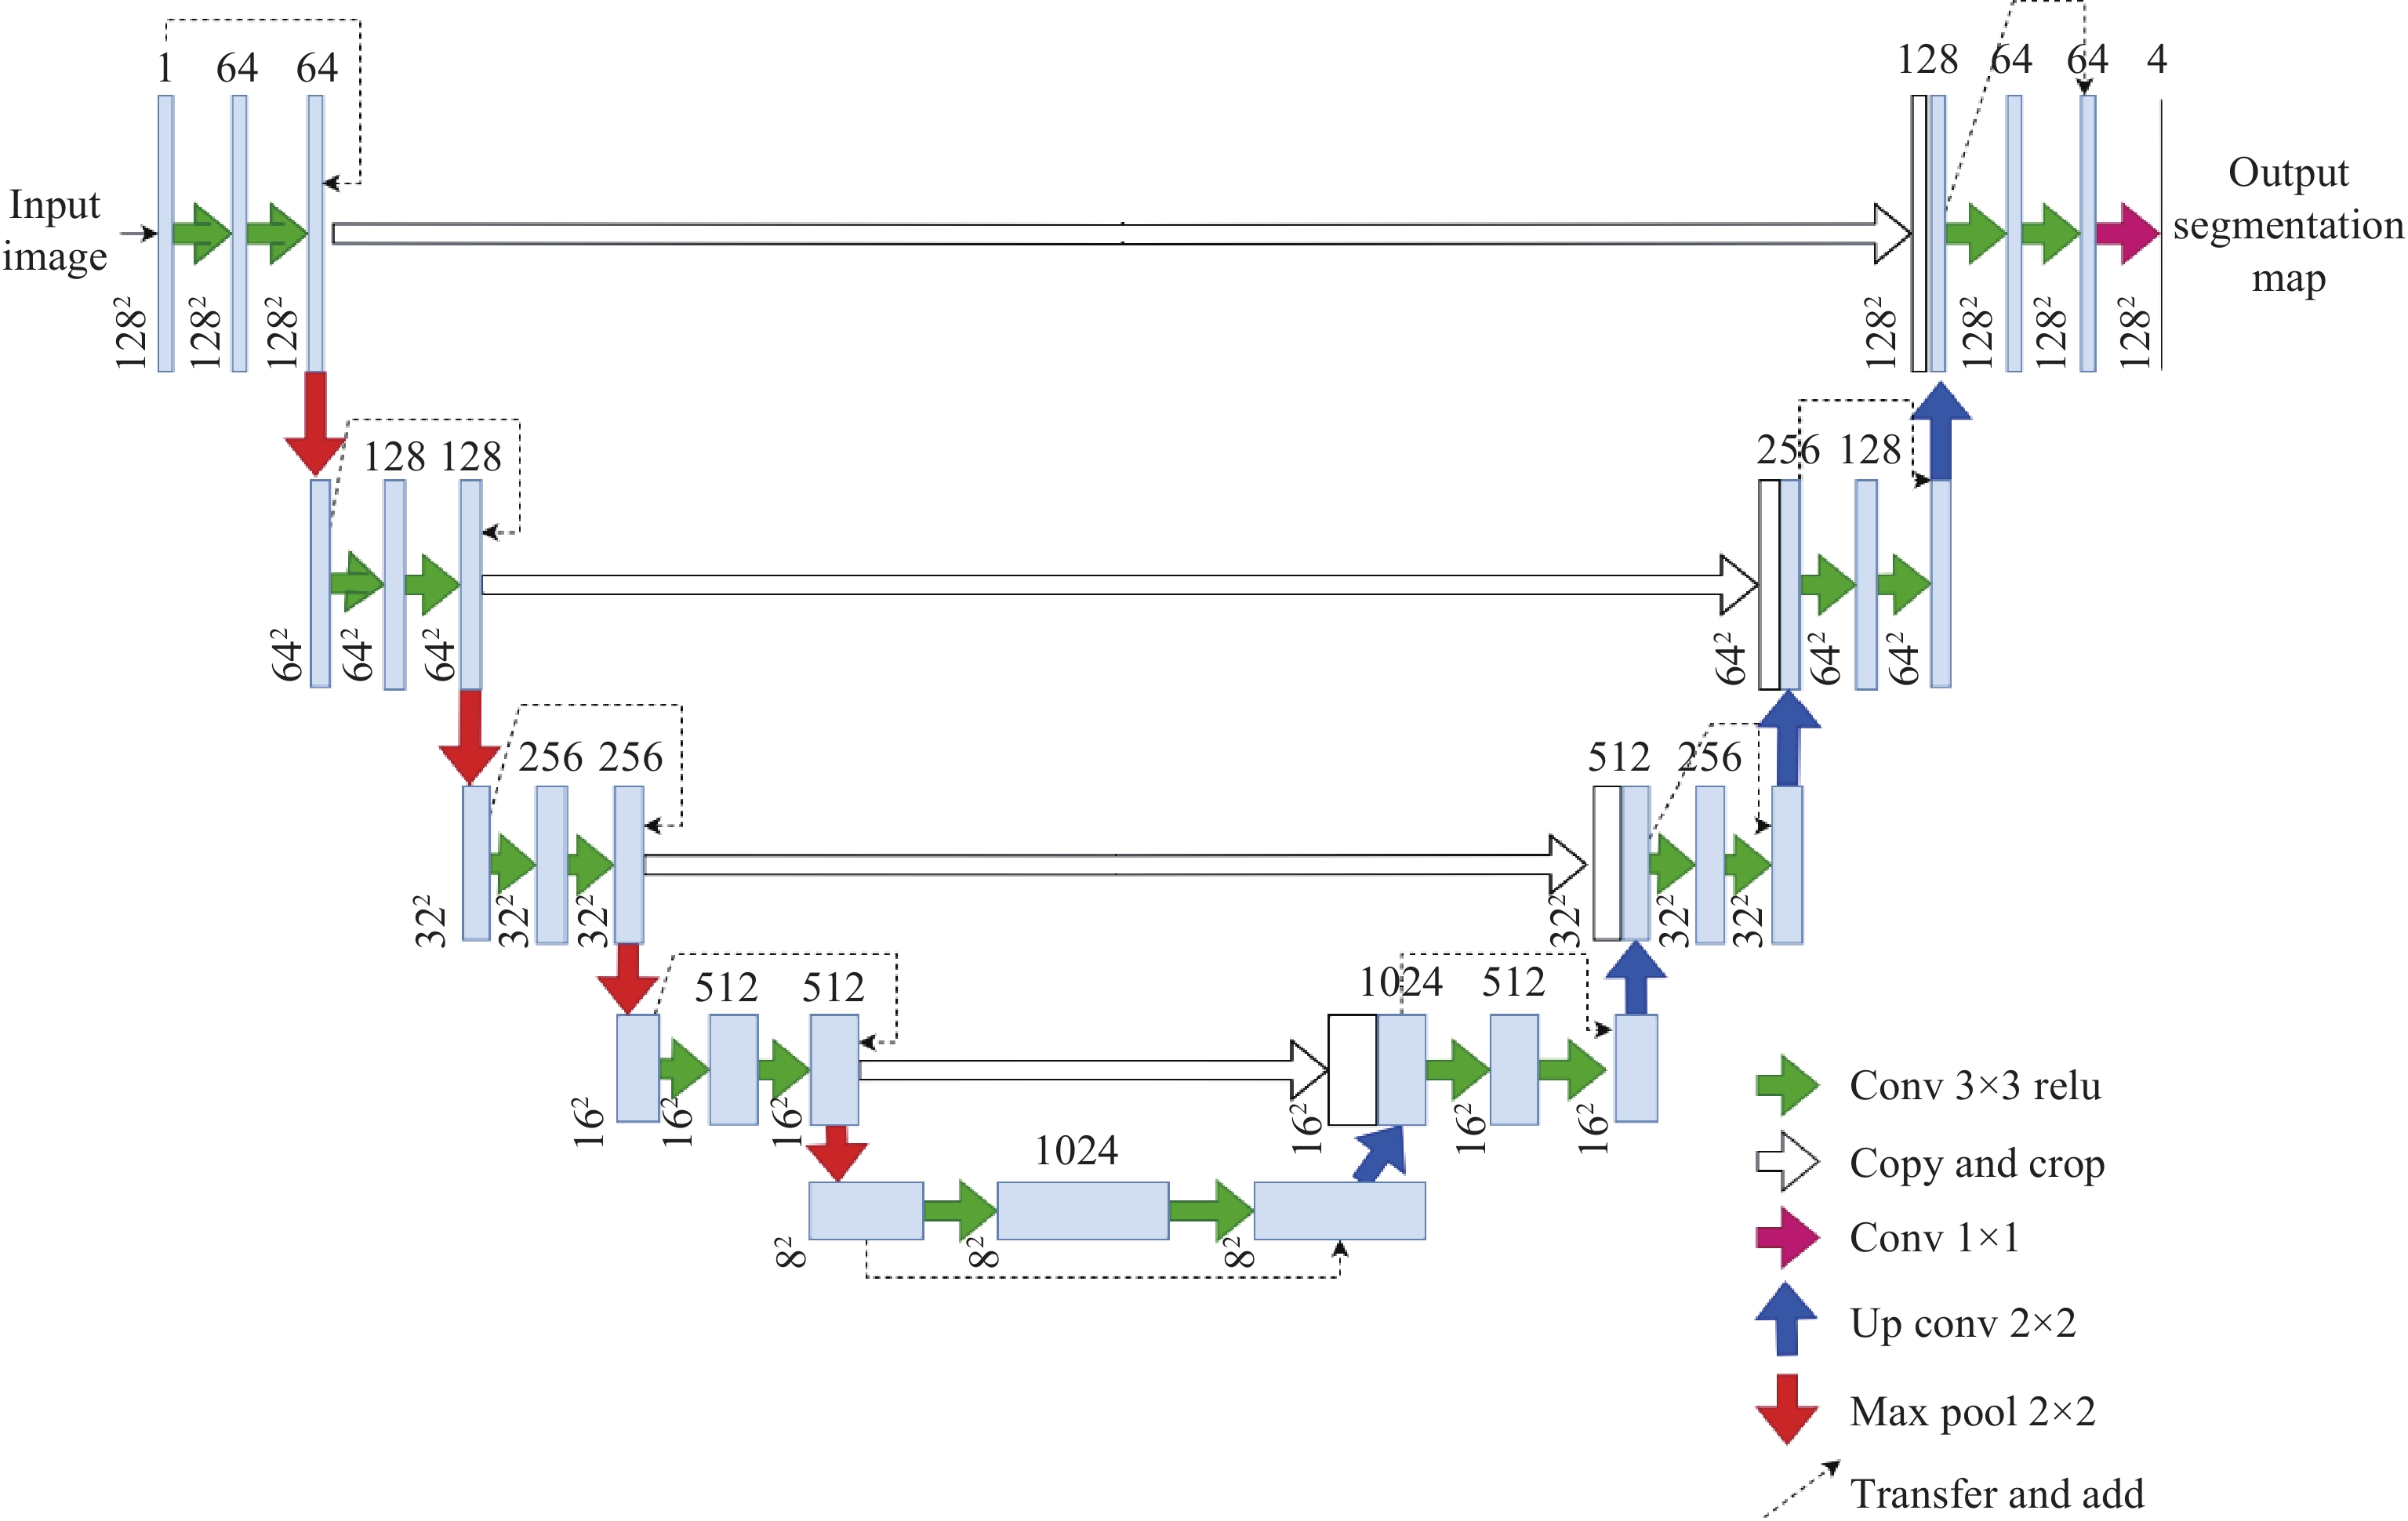
\includegraphics[width=0.6\linewidth]{images/unet.jpg}
          \caption{U-Net Standard Architecture}
          \label{fig:enter-label}
      \end{figure}
\end{frame}

% FEDE
% parlare dei 2 dataset (all'inizio erano 3) + come li abbiamo gestiti (preprocessing + abbiamo ritagliato per salvare risorse + minmax normalizzatione)
% parlare del datset di train locale piccolo da 100 esempi per esperimenti e quello su colab da 1000 esempi per training effettivo

\begin{frame}{Datasets}
    For the purpose of this project, the wind field representations are derived from the ERA5 and VHR--REA datasets.
    \vspace{1em}
        \begin{itemize}
        \justifying
            \item[-] \textbf{ERA5} is a global reanalysis dataset developed by ECMWF, providing hourly data since 1950 at a 0.25° (\textasciitilde31 km) resolution.
            \item[-] \textbf{VHR--REA} is a downscaled regional reanalysis for Italy based on the COSMO model, with a resolution of 2.2 km.
        \end{itemize}
    \vspace{1em}
    Both datasets are aligned temporally (06, 12, 18, 00 UTC) and spatially through reprojection. \\
    \vspace{1em}
    ERA5 acts as the low-resolution input; VHR-REA is used as the high-resolution target for training.
\end{frame}

\begin{frame}{From Global to Surface Reanalysis}
    \centering
    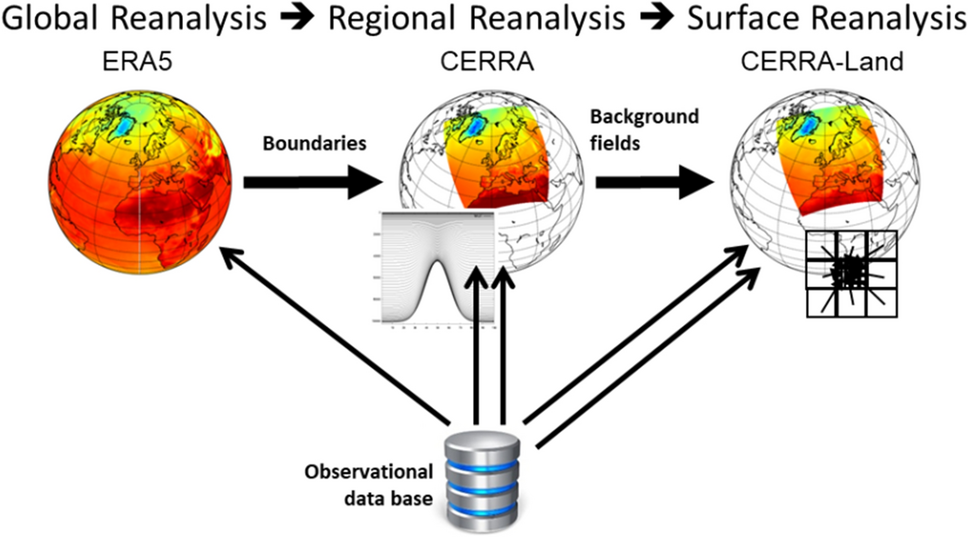
\includegraphics[width=0.6\linewidth]{images/wind_speed.png} \\[2em]
    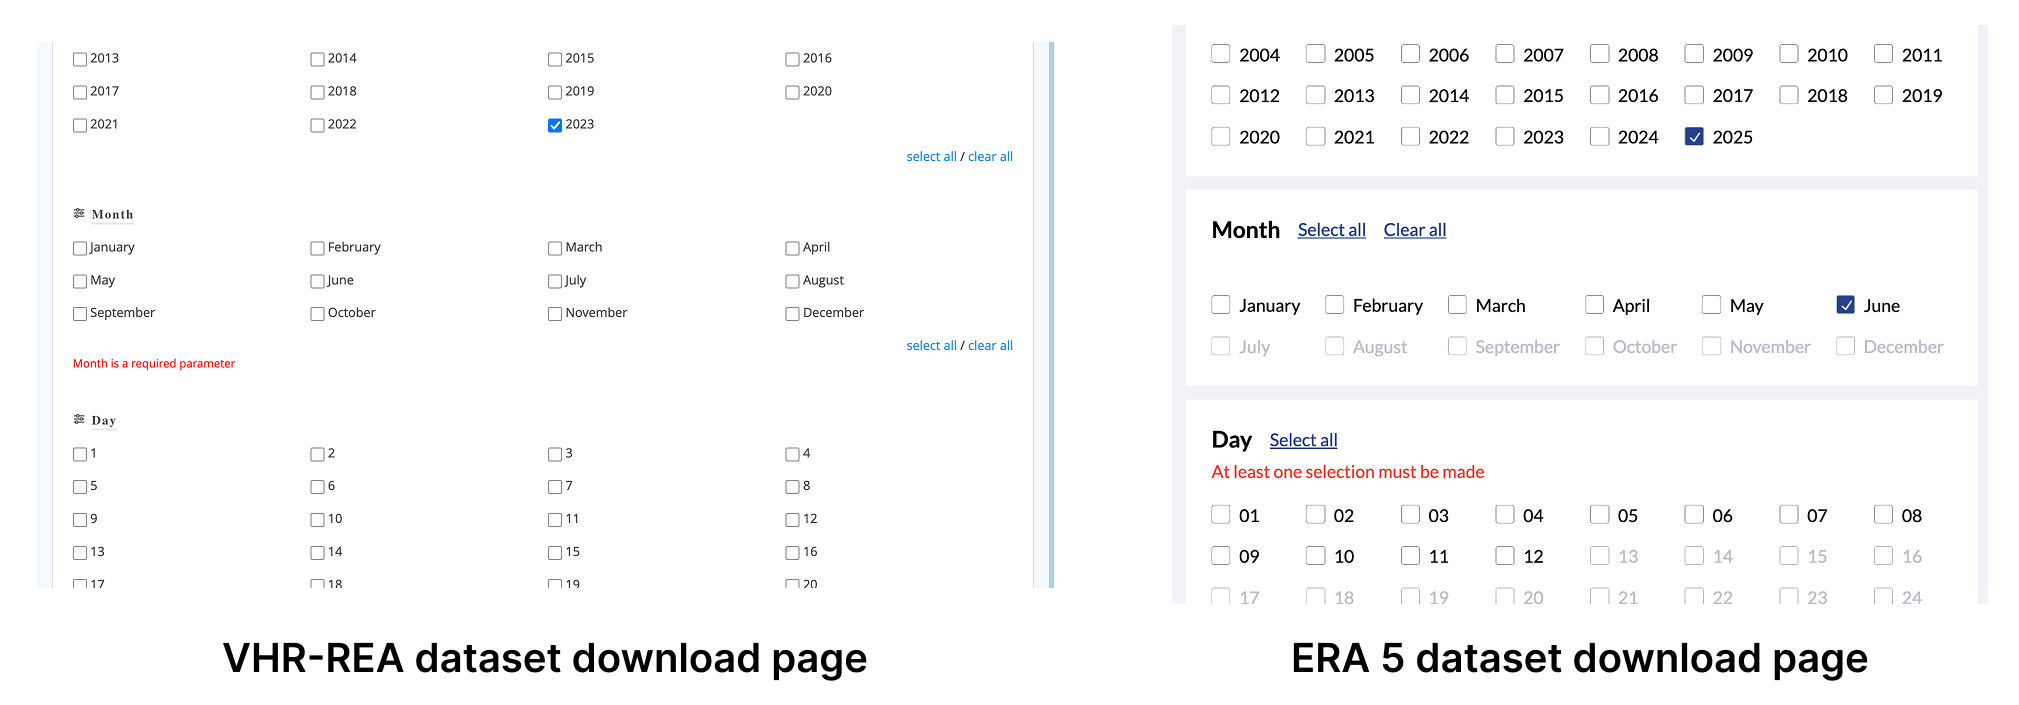
\includegraphics[width=0.9\linewidth]{images/downloadtime.png}
\end{frame}

\begin{frame}{Datasets - ERA5}
\scriptsize
\begin{columns}
    \begin{column}{0.65\textwidth}
        \justifying
        \textbf{ERA5} is a global reanalysis dataset by ECMWF under the Copernicus Climate Change Service (C3S). 
        It offers hourly data from 1950 at 0.25° resolution, replacing the older ERA-Interim.

        \vspace{0.5em}
        Based on 4D-Var data assimilation, ERA5 integrates satellite, radiosonde, buoy, and aircraft observations, covering atmosphere, land, and ocean.

        \vspace{0.5em}
        In this project, we use surface wind components \texttt{u10} and \texttt{v10} as low-resolution inputs for super-resolution modeling.
    \end{column}

    \begin{column}{0.35\textwidth}
        \centering
        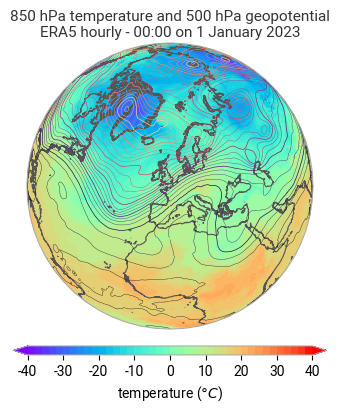
\includegraphics[width=\linewidth]{images/overview-detail_67e6d1d5ac470ee33ae510a76a2fe3c1c67a7f1fdd4c040a333969fe0b11f76f.png}
    \end{column}
\end{columns}
\end{frame}

\begin{frame}{Datasets - VHR-REA}
\justifying
\scriptsize
\begin{wrapfigure}{r}{0.4\textwidth}
    \centering
    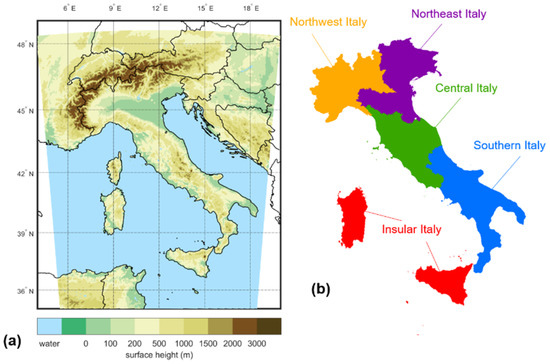
\includegraphics[width=0.38\textwidth]{images/data-06-00088-g001-550.jpg}
    \caption{VHR--REA spatial coverage over Northern Italy}
\end{wrapfigure}

\textbf{VHR--REA (Very High Resolution ReAnalysis)} is produced by CMCC via dynamic downscaling of ERA5 using the COSMO model. It reaches a spatial resolution of ~2.2 km, resolving convection in complex terrain.

\vspace{0.5em}
This dataset is designed for high-resolution applications such as hydrology, renewable energy, and urban climate.

\vspace{0.5em}
\begin{itemize}
    \item[-] Used as high-resolution target for training.
    \item[-] Temporal coverage: 4 times daily for one full year.
\end{itemize}
\end{frame}


\begin{frame}[fragile]
\frametitle{ERA5 \& VHR--REA: Regridding Pipeline}

\tiny
\begin{columns}
\begin{column}{0.42\textwidth}
\textbf{ERA5 \textrightarrow{} VHR Reprojection Strategy}
\begin{itemize}
    \item[-] ERA5 loaded with Dask chunking
    \item[-] Target grid built from concatenated VHR quarters
    \item[-] Bilinear regridding using \texttt{xesmf}
    \item[-] Reuse of interpolation weights (caching)
    \item[-] Post-rechunking to control memory usage
\end{itemize}

\vspace{0.3cm}

\textbf{Data Output \& Performance}
\begin{itemize}
    \item[-] Lazy NetCDF writing with Dask
    \item[-] Compute triggered with progress bar
    \item[-] Output aligned with VHR spatial resolution
\end{itemize}
\end{column}

\begin{column}{0.58\textwidth}
\begin{lstlisting}[language=Python, basicstyle=\ttfamily\tiny]
# Step 1: Load ERA5 with chunks
era5 = xr.open_dataset("era5.nc",
    chunks={"time": 10, "lat": 300, "lon": 300})

# Step 2: Load and combine VHR target grid
vhr = xr.concat([
    xr.open_dataset("vhr_q1.nc"),
    xr.open_dataset("vhr_q2.nc")
], dim="time")

# Step 3: Create bilinear regridder
regridder = xe.Regridder(
    era5, vhr, method="bilinear",
    filename="weights.nc")

# Step 4: Apply regridding + rechunk
output = regridder(era5).chunk({
    "time": 10, "rlat": 100, "rlon": 100})

# Step 5: Save with progress bar
with ProgressBar():
    output.to_netcdf("regridded.nc")
\end{lstlisting}
\end{column}
\end{columns}
\end{frame}


\begin{frame}[fragile]
\frametitle{Preprocessing}
\scriptsize
\begin{columns}
    % Colonna sinistra: testo
    \begin{column}{0.55\textwidth}
        \textbf{Spatial Alignment \& Patch Extraction}
        \begin{itemize}
            \item[-] Center crop to 224×224 pixel patches
            \item[-] Temporal synchronization verification
            \item[-] Channel-wise data stacking (u10, v10 components)
            \item[-] Custom PyTorch Dataset implementation
        \end{itemize}

        \textbf{Data Pipeline Architecture}
        \begin{itemize}
            \item[-] ItalyWeatherDataset class for paired data loading
            \item[-] Automatic temporal alignment checking
            \item[-] Flexible normalizer integration
            \item[-] Memory-efficient batch processing
        \end{itemize}

        \textbf{Quality Assurance}
        \begin{itemize}
            \item[-] Index bounds verification
            \item[-] Consistent tensor dimensions
            \item[-] Error handling for misaligned datasets
        \end{itemize}
    \end{column}

    % Colonna destra: codice
    \begin{column}{0.45\textwidth}
        \begin{lstlisting}[language=Python, basicstyle=\ttfamily\tiny]
def extract_region(self, data_tensor):
    patch_h, patch_w = (224, 224)
    _, h, w = data_tensor.shape
    x = (w - patch_w) // 2
    y = (h - patch_h) // 2
    return data_tensor[:, 
                      y:y+patch_h, 
                      x:x+patch_w]

def __getitem[-]__(self, idx):
    era_slice = self.era5_dataset.isel(valid_time=idx)
    era_arrays = [era_slice[v].values 
                  for v in self.ERA5_VARIABLES]
    era_tensor = torch.from_numpy(
        np.stack(era_arrays, axis=0)).float()
    era_tensor = self.extract_region(era_tensor)

    if self.era5_normalizer:
        era_tensor = self.era5_normalizer.normalize(era_tensor)
        \end{lstlisting}
    \end{column}
\end{columns}
\end{frame}


\begin{frame}[fragile]
\frametitle{Normalization \& Coordinate Transformation}

\tiny
\begin{columns}
\begin{column}{0.4\textwidth}
\textbf{MinMax Normalization Strategy}
\begin{itemize}
    \item[-] Training-based statistics computation
    \item[-] Per-channel normalization across spatial dimensions
    \item[-] Feature range scaling to [0, 1]
    \item[-] Epsilon handling for division-by-zero cases
    \item[-] Serializable normalizer objects
\end{itemize}

\vspace{0.3cm}

\textbf{Coordinate System Transformation}
\begin{itemize}
    \item[-] \textbf{Option 1}: Cartesian coordinates (u, v)
    \item[-] \textbf{Option 2}: Polar coordinates (magnitude, direction)
    \item[-] $magnitude = \sqrt{u^2 + v^2}$
    \item[-] $direction = 180° + \frac{180°}{\pi} \arctan2(-u, -v) \bmod 360°$
\end{itemize}

\vspace{0.3cm}

\textbf{Dataset Management}
\begin{itemize}
    \item[-] 80-20 train-test split with fixed seed (42)
    \item[-] Separate normalization preservation
    \item[-] Batch processing with memory optimization
\end{itemize}
\end{column}

\begin{column}{0.6\textwidth}

\begin{lstlisting}[language=Python, basicstyle=\ttfamily\tiny]
class MinMaxNormalizer:
    def compute_stats(self, data_tensor):
        # Min/max per channel across (N,H,W) dims
        self.min_val = data_tensor.amin(
            dim=(0, 2, 3), keepdim=True)
        self.max_val = data_tensor.amax(
            dim=(0, 2, 3), keepdim=True)
        
        # Handle division by zero
        diff = self.max_val - self.min_val
        epsilon = 1e-7
        self.max_val[diff < epsilon] = \
            self.min_val[diff < epsilon] + epsilon
    def normalize(self, x):
        return (x - self.min_val) / \
               (self.max_val - self.min_val)

# Coordinate transformation to polar
if COORDINATES == "1":
    u_squared = tensor[0, :, :]**2
    v_squared = tensor[1, :, :]**2
    magnitude = torch.sqrt(u_squared + v_squared)
    direction = (180 + (180/math.pi) * 
                torch.atan2(-u_squared, -v_squared)) % 360
    tensor = torch.stack([magnitude, direction], axis=0)
\end{lstlisting}
\end{column}
\end{columns}

\end{frame}

% --- MATTEO ---
% spiegare che modello abbiamo usato (upconv vs bilinear upsampling) + come abbiamo scelto la loss + come abbiamo scelto gli iperparametri
% [x] panoramica generale sul modello
% [x] upconv vs bilinear upsampling
% [x] loss
% [x] iperparametri (tabella)
\begin{frame}{Model and hyperparameters - General differences}
    \begin{columns}
        \begin{column}{0.45\textwidth}
            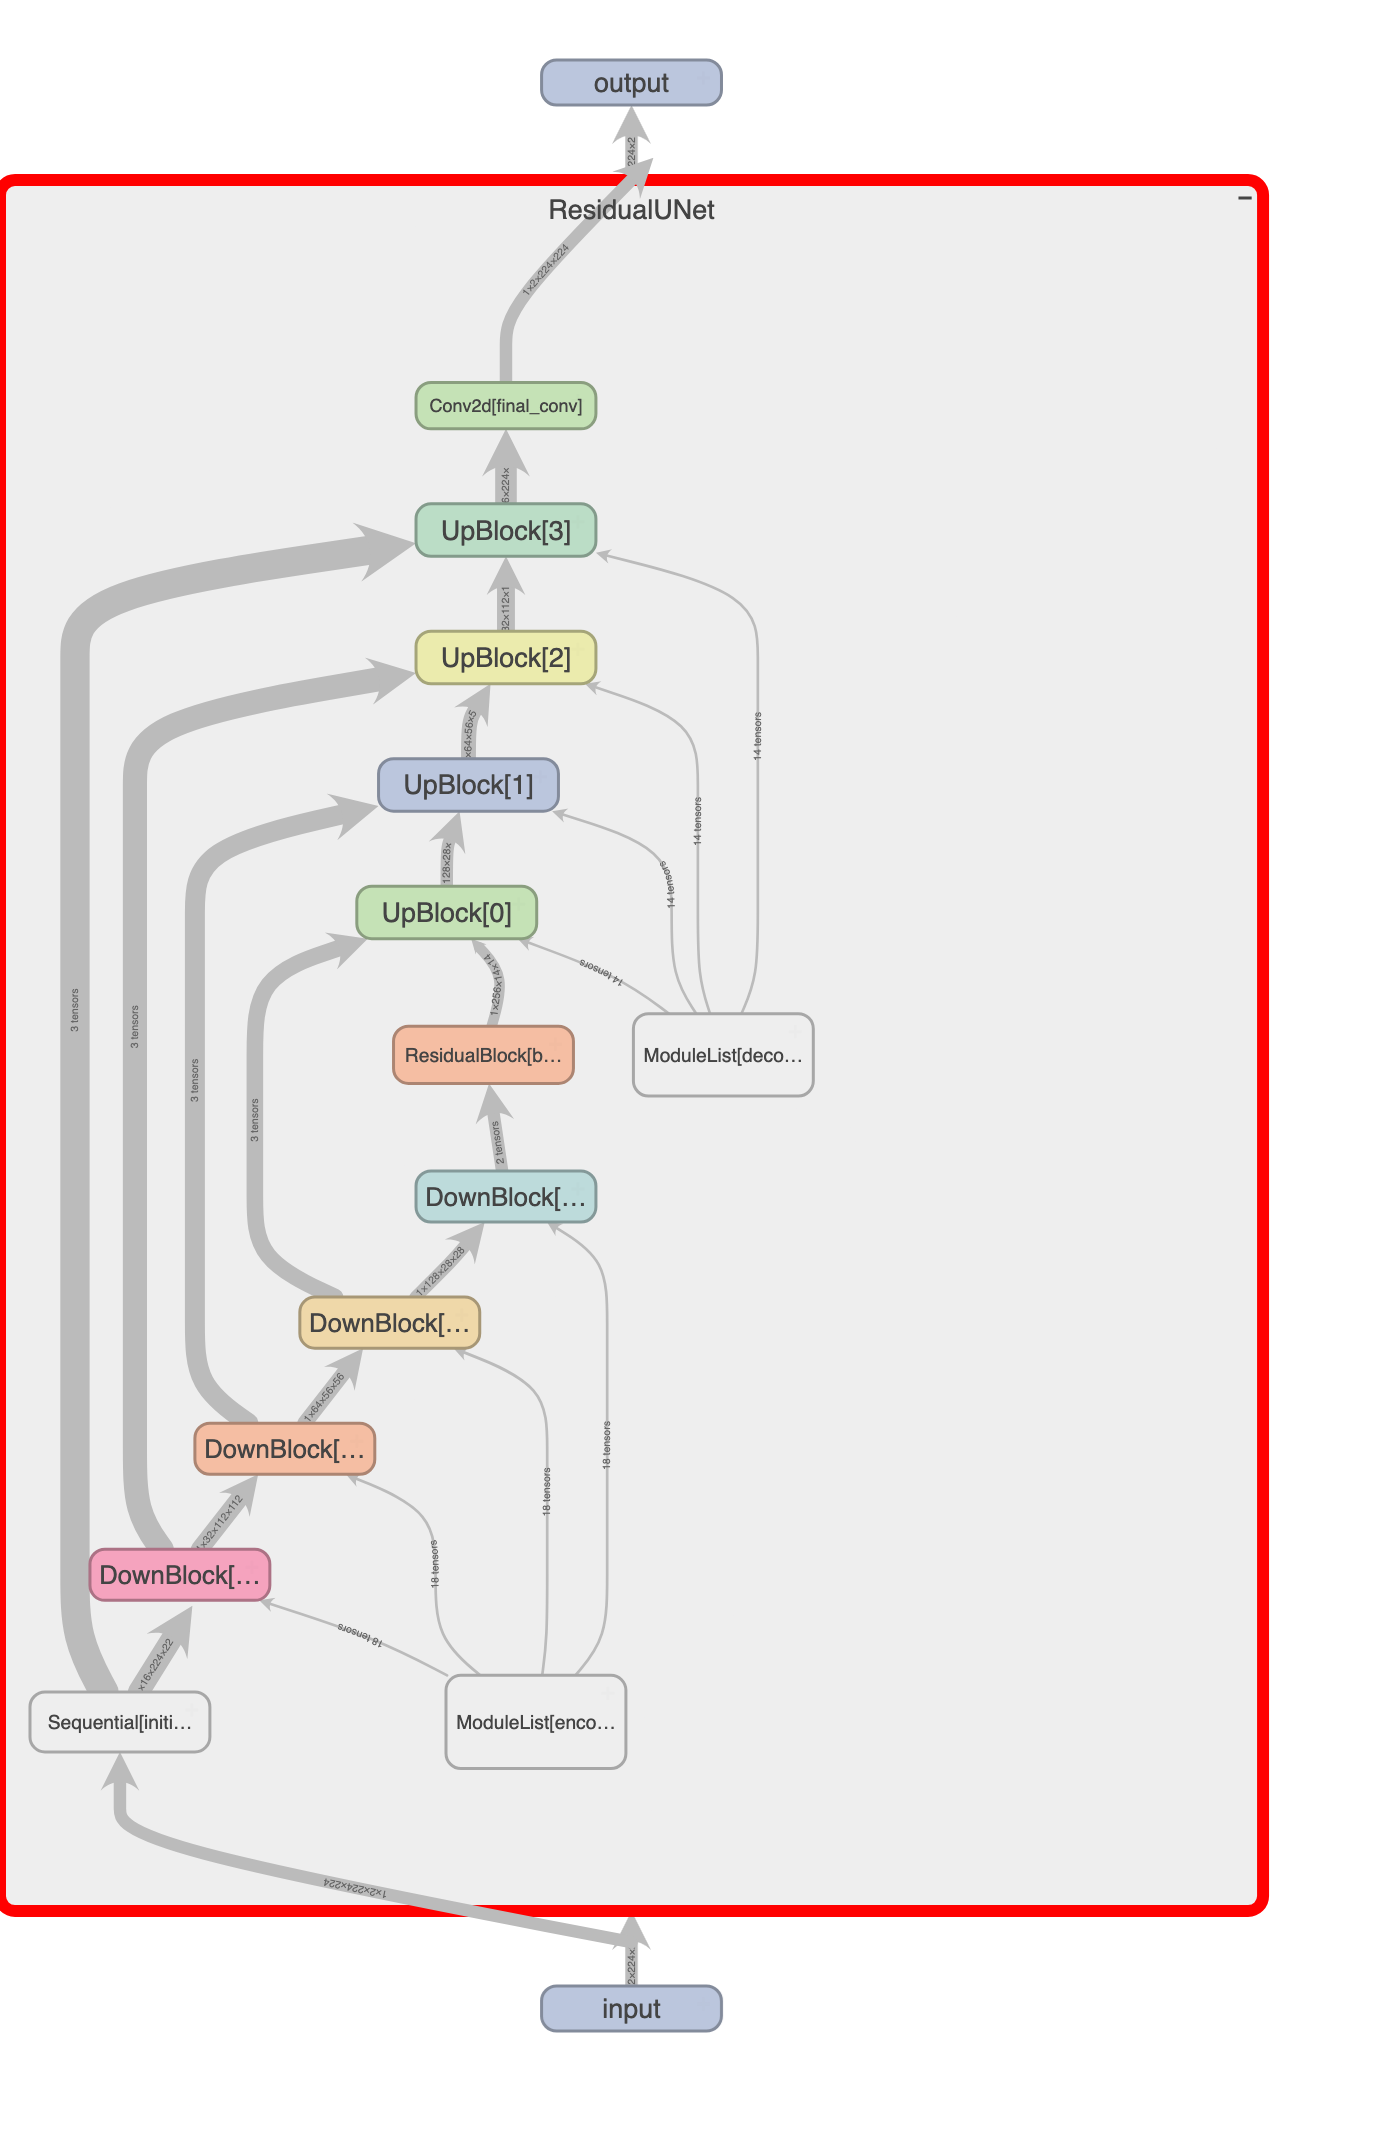
\includegraphics[width=0.6\textheight]{images/unet_experiment_graph.png}
        \end{column}
        \begin{column}{0.55\textwidth}
            Interesting points in our implementation:
            \begin{itemize}
                \item[-] \texttt{Conv2d} with \texttt{stride=2} for downsampling.
                \item[-] \texttt{BatchNorm} to reduce internal covariate shift. This improves speed and stability of the training.
            \end{itemize}
            But there's more...
        \end{column}
    \end{columns}
\end{frame}

\begin{frame}{Model and hyperparameters - Transposed vs Bilinear}

    \begin{table}[ht]
        \centering
        \scriptsize
        \begin{tabular}{|l|l|l|l|l|}
        \hline
        \textbf{Network Type} & \textbf{Parameters Count} & \textbf{Training Time} & \textbf{Test Loss} & \textbf{Test SSIM} \\
        \hline
        Transposed Conv & 13,041,922 (13.0 M) & 54:03 16.22s/it & 0.19775 & 0.70910 \\
        Bilinear Interp & 3,607,586 (3.6 M) & 08:04 2.42s/it & 0.17166 & 0.74983 \\
        \hline
        \end{tabular}
        \caption{Comparison of bilinear interpolation vs transposed convolution.}
        \label{tab:network_comparison}
    \end{table}
\end{frame}

\begin{frame}{Model and hyperparameters - Loss}
    Even the best model couldn't get decent results with the suggested MSE loss, so we adopted a combined loss approach
    \begin{columns}
        \column{0.5\textwidth}
            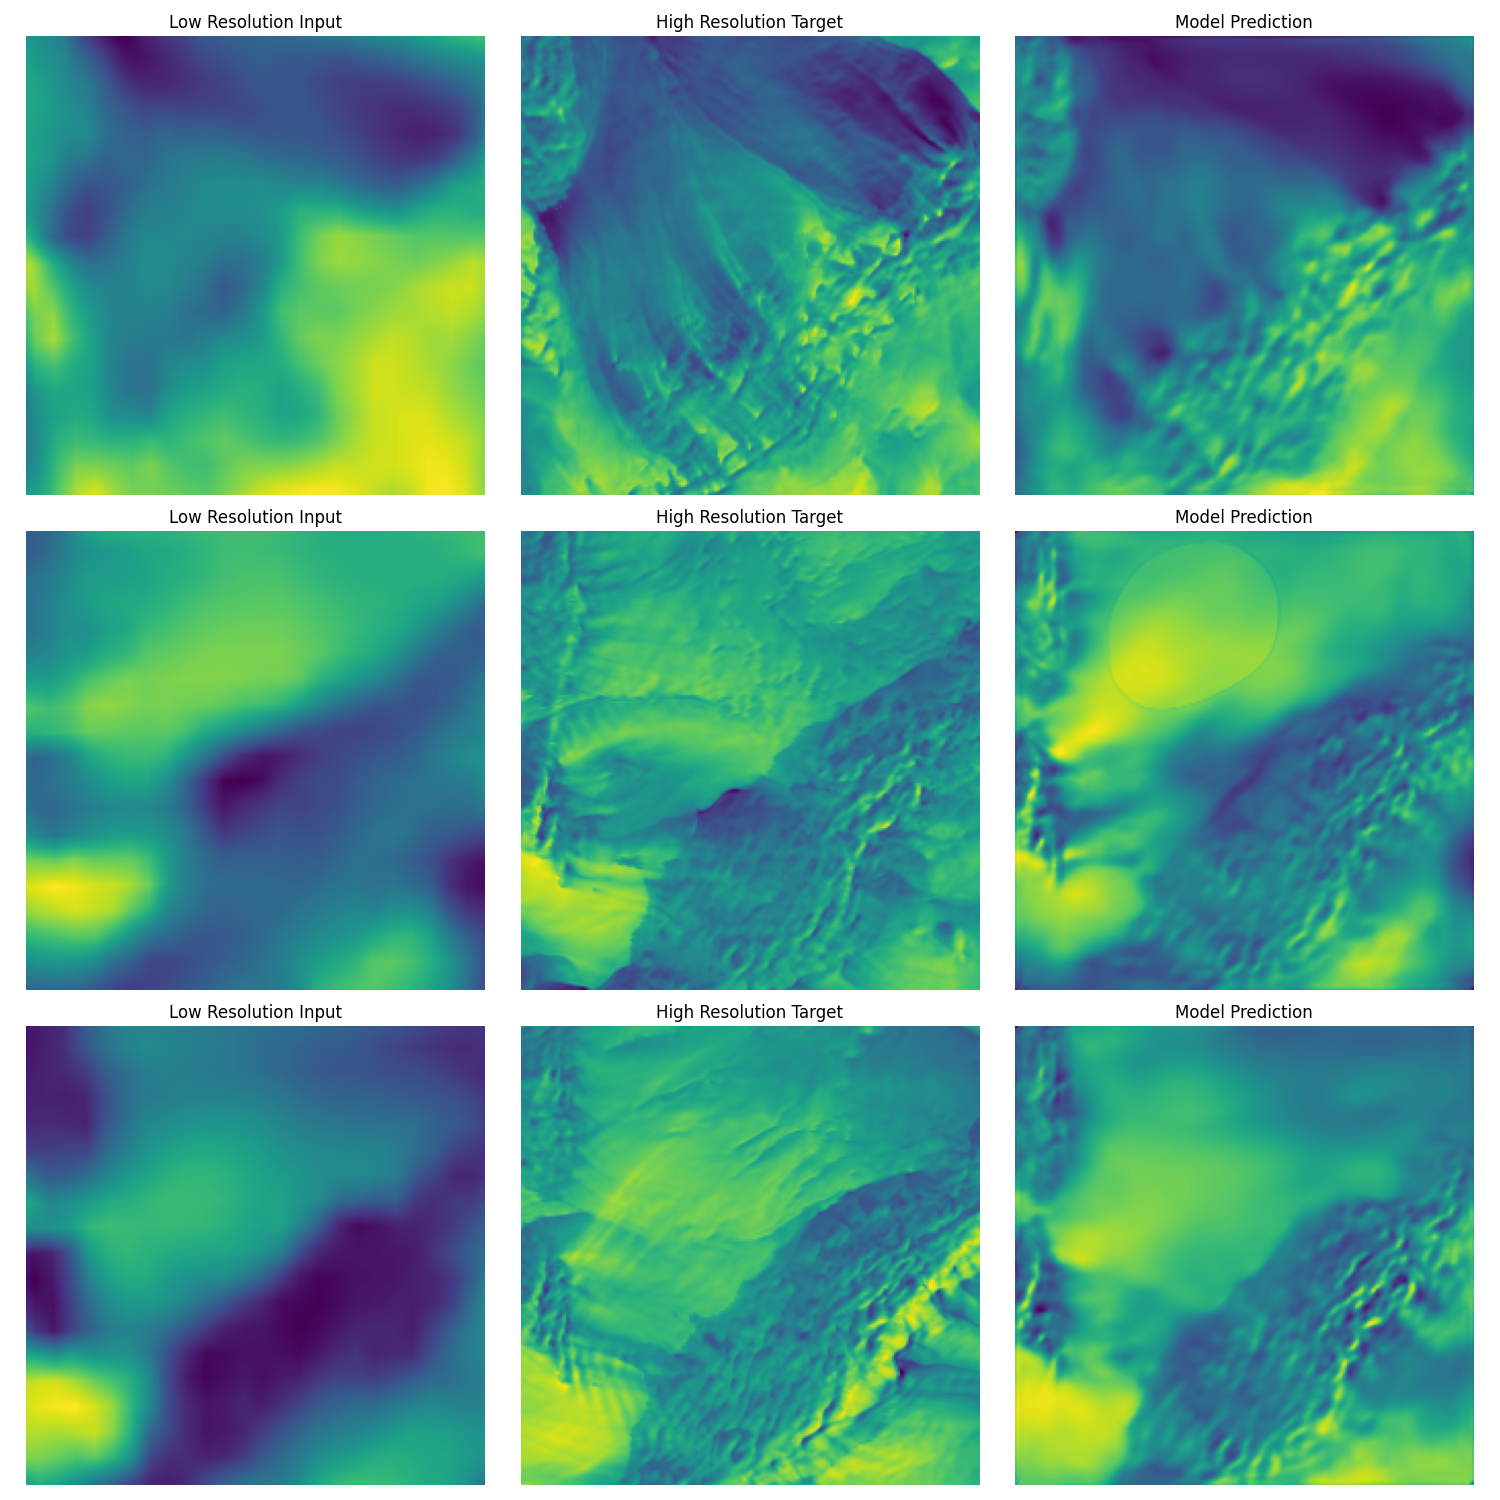
\includegraphics[width=\linewidth]{images/unet_vectors_l1ssim_loss_200_epochs_4_batch_1em3_lr_1em5_weightdecay.png}
            \newline
            \centering \small L1 + SSIM loss. SSIM: \texttt{0.7556}
        \column{0.5\textwidth}
            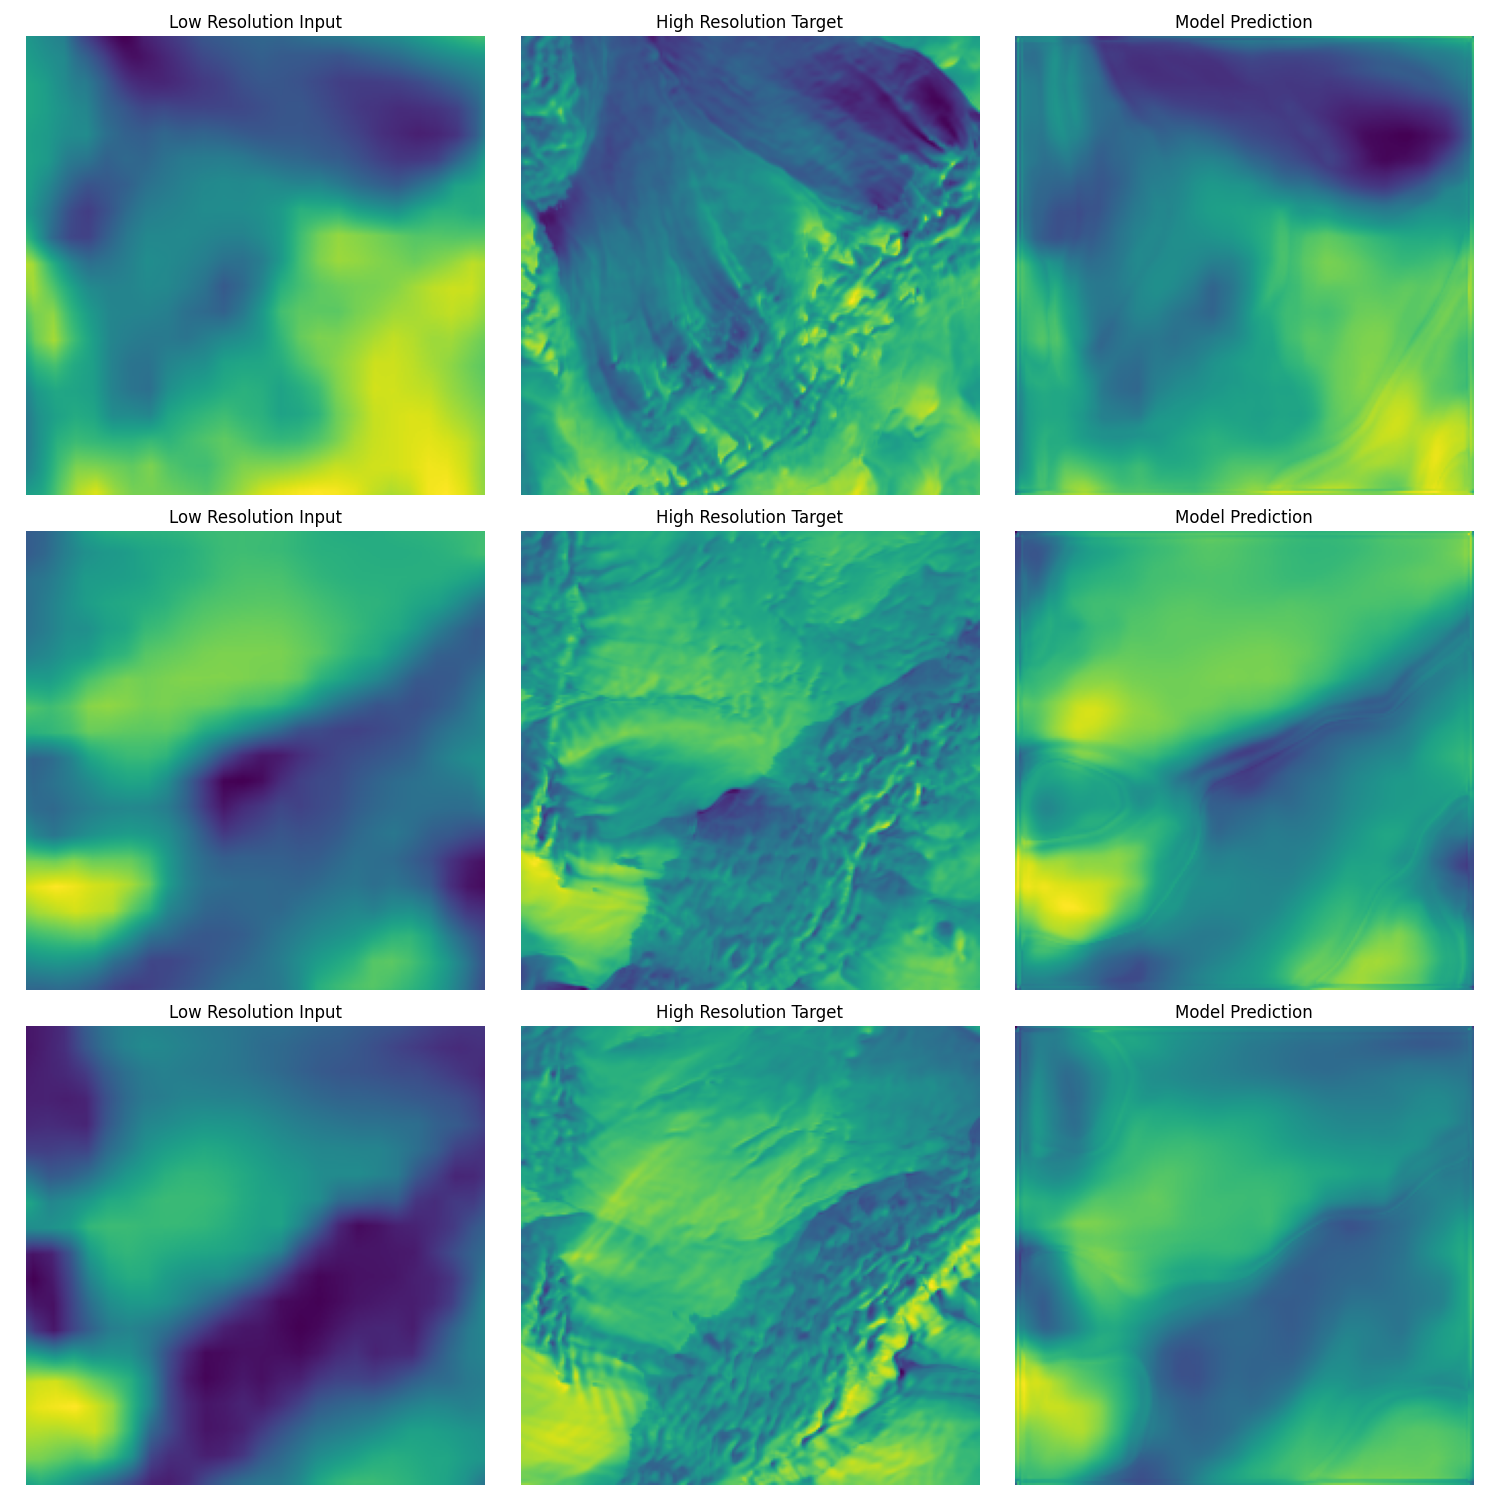
\includegraphics[width=\linewidth]{images/unet_vectors_mse_loss_200_epochs_4_batch_1em3_lr_1em5_weightdecay.png}
            \newline
            \centering \small MSE loss. SSIM: \texttt{0.7022}
    \end{columns}
\end{frame}

\begin{frame}[fragile]{Model and hyperparameters - Loss}
    \begin{lstlisting}
class L1SSIMLoss(nn.Module):
    def __init__(self, alpha=0.85, ssim_window_size=11, ssim_data_range=1.0, ssim_channel=1):
        super(L1SSIMLoss, self).__init__()
        self.alpha = alpha
        self.l1_loss = nn.L1Loss() # Mean Absolute Error
        self.ssim_loss_fn = SSIMLoss(window_size=ssim_window_size, data_range=ssim_data_range, channel=ssim_channel)

    def forward(self, y_pred, y_true):
        ssim_val_loss = self.ssim_loss_fn(y_pred, y_true)
        l1_val_loss = self.l1_loss(y_pred, y_true)
        
        combined_loss = self.alpha * ssim_val_loss + (1 - self.alpha) * l1_val_loss
        return combined_loss
    \end{lstlisting}
\end{frame}

\begin{frame}{Model and hyperparameters - Hyperparameters}
    \begin{table}[ht]
        \centering
        \normalsize
        \resizebox{\textwidth}{!}{%
        \begin{tabular}{|c|c|c|c|c|c|c|c|c|}
        \hline
        \textbf{Channels} & \textbf{Epochs} & \textbf{Loss} & \textbf{Batch Size} & \textbf{LR} & \textbf{LR Scheduler} & \textbf{Weight Decay} & \textbf{Test Loss} & \textbf{Test SSIM} \\
        \hline
        {[}32, 64, 128{]} & 200 & L1 + SSIM & 8 & 1.00E-03 & NO & 1.00E-05 & 0.19090 & 0.71990 \\
        {[}16, 32, 64, 128{]} & 200 & L1 + SSIM & 8 & 1.00E-03 & NO & 1.00E-05 & 0.17700 & 0.74170 \\
        {[}16, 32, 64, 128, 256{]} & 300 & L1 + SSIM & 8 & 1.00E-03 & NO & 1.00E-05 & \textbf{0.16768} & \textbf{0.75555} \\
        {[}16, 32, 64, 128, 256{]} & 300 & MSE + SSIM & 8 & 1.00E-03 & NO & 1.00E-05 & \underline{0.15464} & \underline{0.75391} \\
        {[}16, 32, 64, 128, 256{]} & 300 & MSE & 8 & 1.00E-03 & NO & 1.00E-05 & 0.00327 & 0.70218 \\
        {[}16, 32, 64, 128, 256, 512{]} & 300 & L1 + SSIM & 8 & 1.00E-03 & NO & 1.00E-05 & 0.19207 & 0.71774 \\
        {[}16, 32, 64, 128, 256, 512{]} & 300 & L1 + SSIM & 8 & 1.00E-03 & YES & 1.00E-05 & 0.19207 & 0.71774 \\
        \hline
        \end{tabular}
        }
        \caption{Performance comparison of different network configurations. Best and runner-up models are highlighted in bold and underline, respectively.}
    \end{table}
\end{frame}

% --- MATTEO ---
% [x] curve di training
\begin{frame}[fragile]{Local Training - Loss and SSIM curves}
    Training curves for the best model on local data (loss and SSIM):
    \newline
    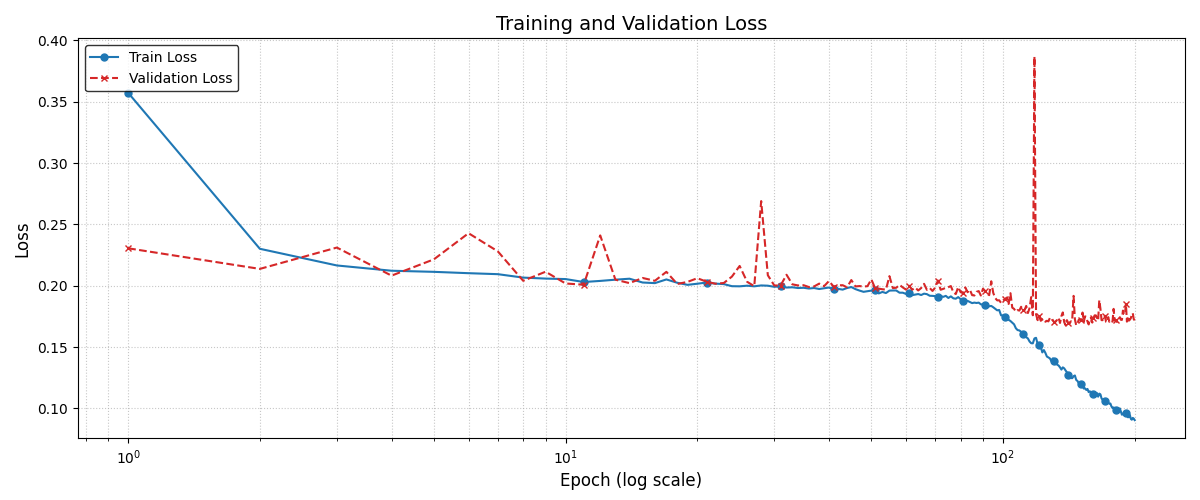
\includegraphics[width=0.7\linewidth]{images/local_loss_curve.png}
    \newline
    \small Loss curve 
    \newline
    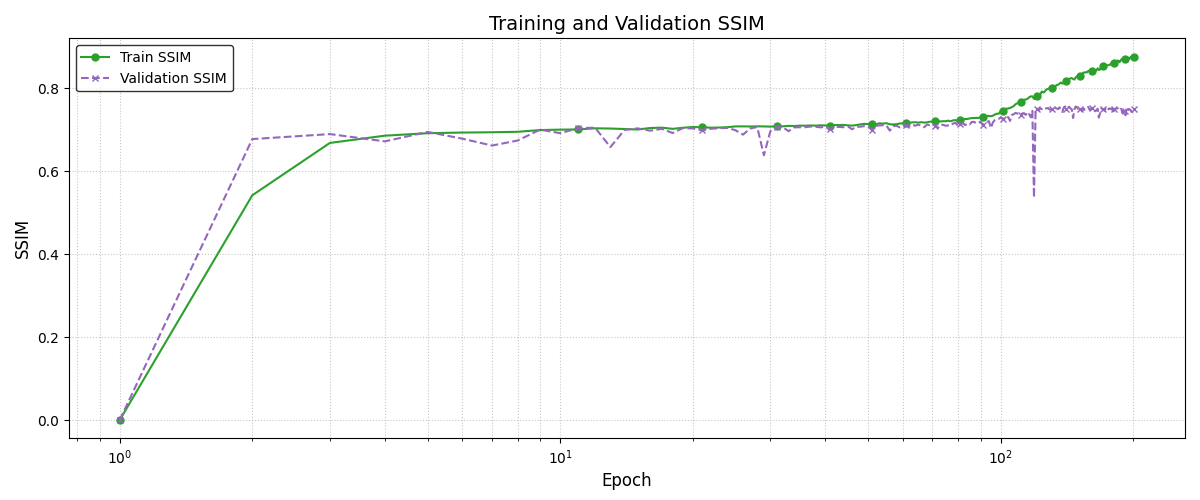
\includegraphics[width=0.7\linewidth]{images/local_ssim_curve.png}
    \newline
    \small SSIM curve 
\end{frame}

\begin{frame}{Colab Training - Difference with Local data}
    \begin{columns}
        \column{0.5\textwidth}
            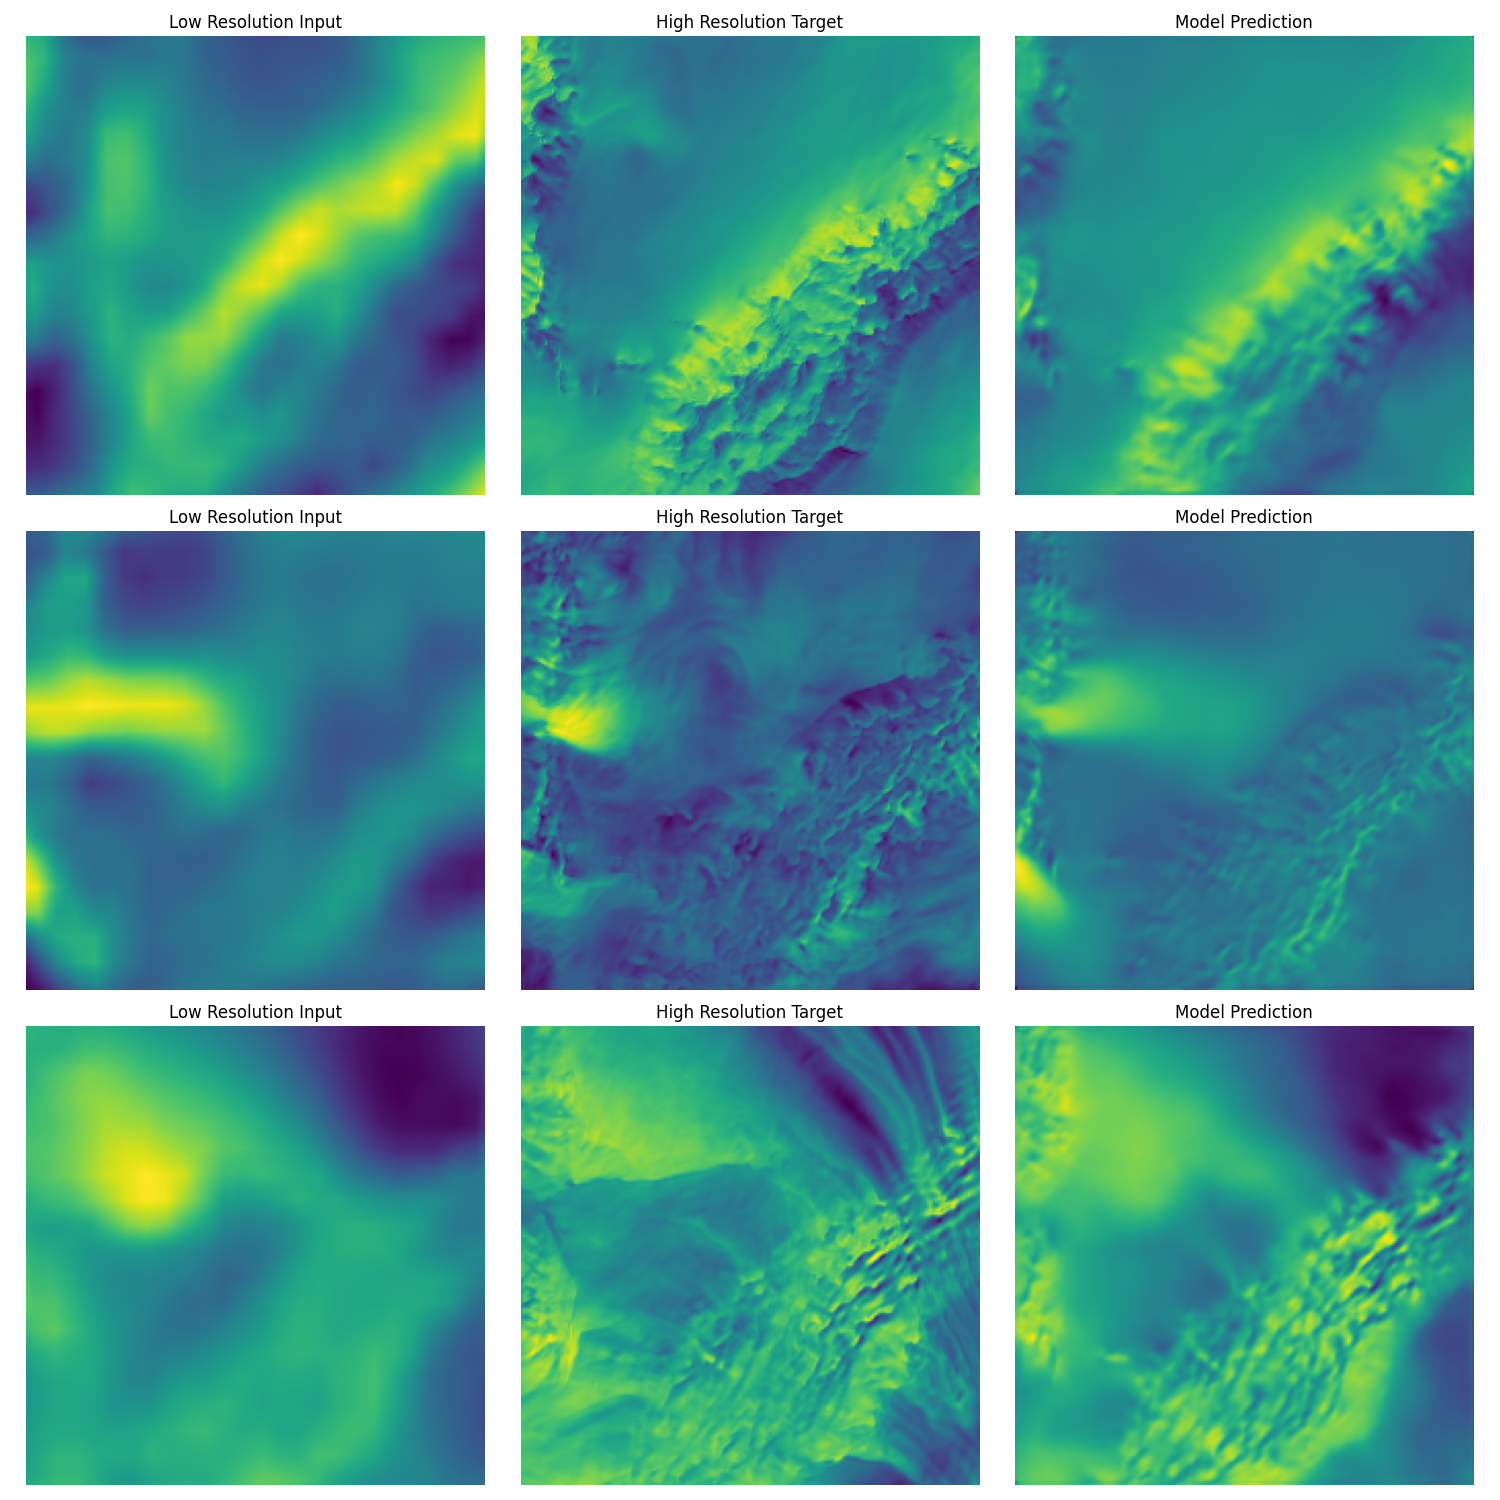
\includegraphics[width=\linewidth]{images/colab_vector_unet_L1SSIM_loss_300_epochs_8_batch_1em3_lr_1em5_weightdecay_best.pt.png}
            \newline
            \centering \small Colab data. SSIM: \texttt{0.84483}
        \column{0.5\textwidth}
            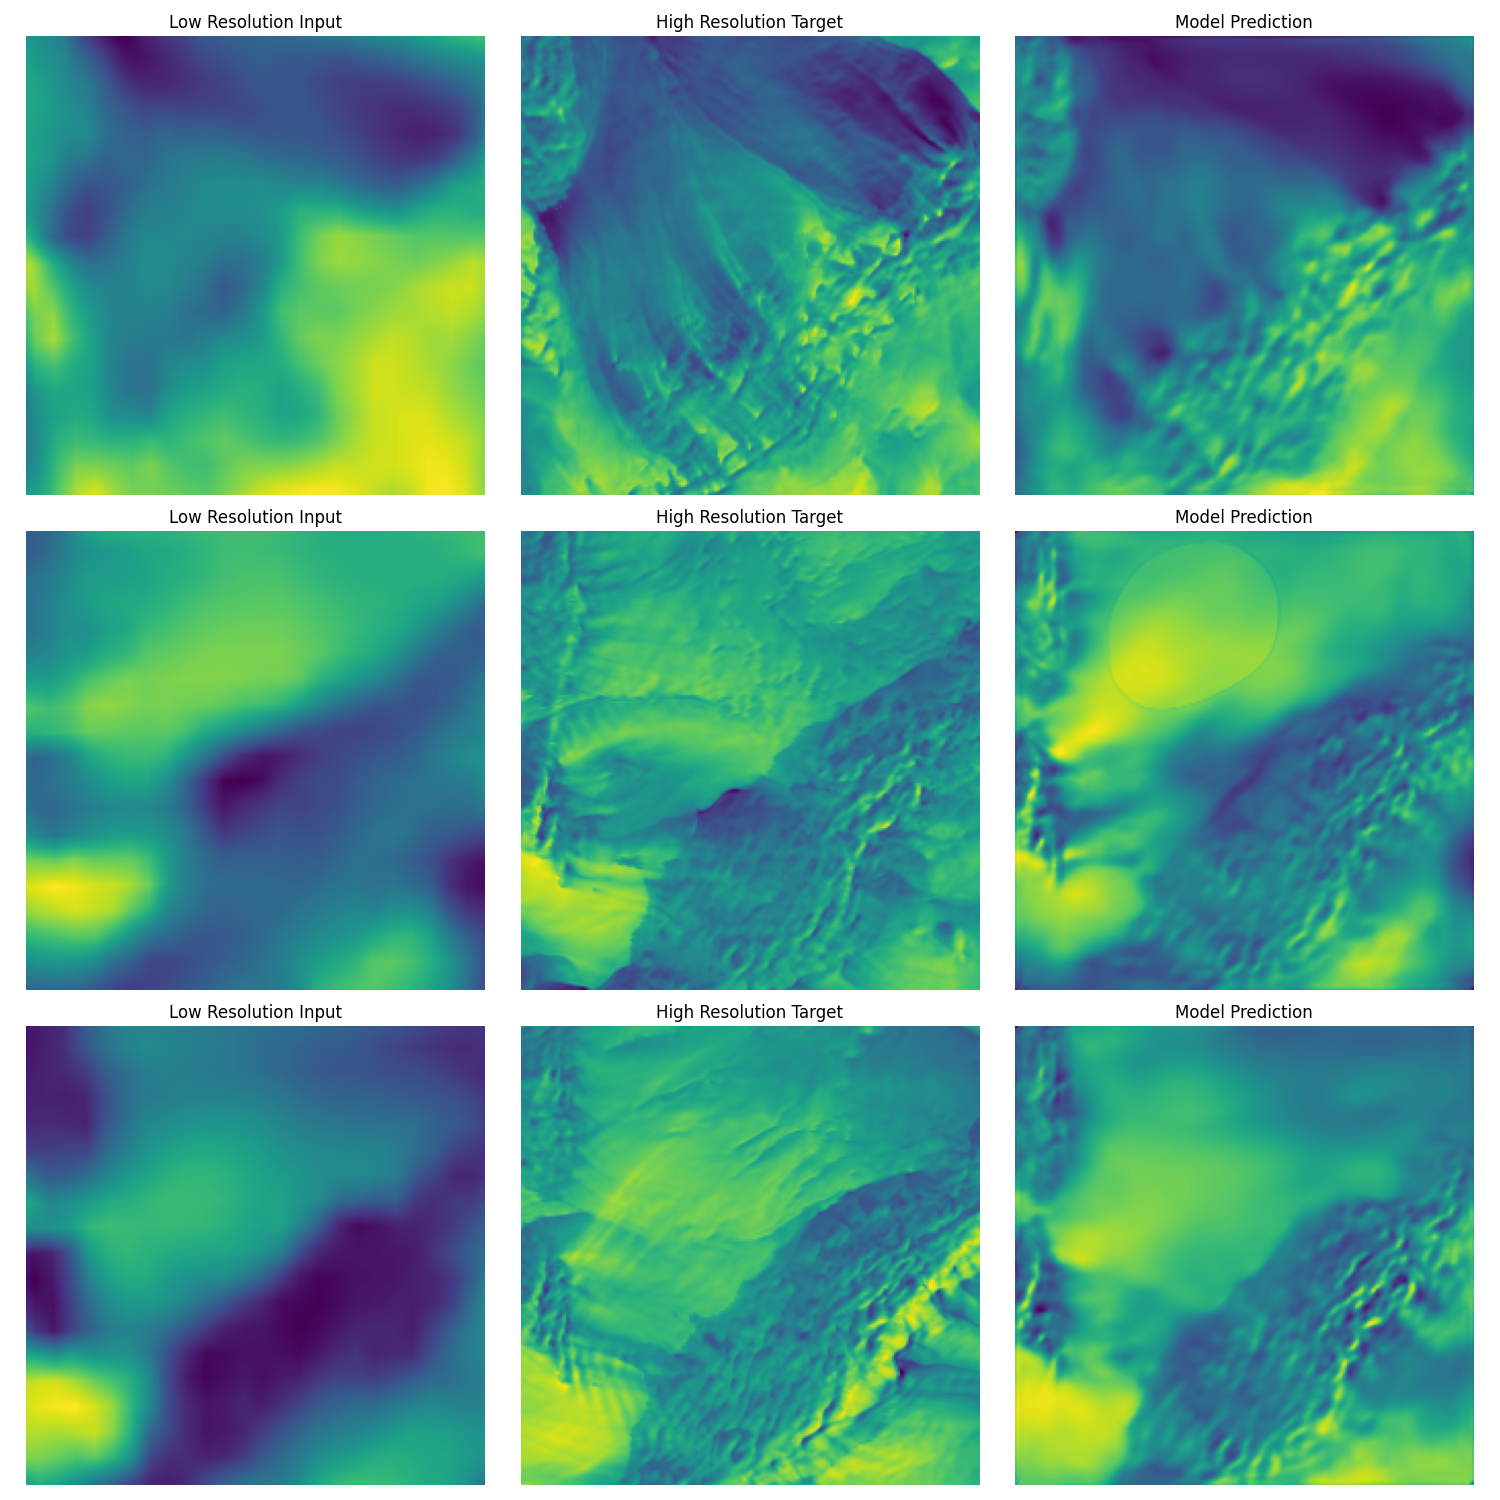
\includegraphics[width=\linewidth]{images/unet_vectors_l1ssim_loss_200_epochs_4_batch_1em3_lr_1em5_weightdecay.png}
            \newline
            \centering \small Local data. SSIM: \texttt{0.7556}
    \end{columns}
\end{frame}

\begin{frame}[fragile]{Colab Training - Loss and SSIM curves}
    Training curves for the best model on colab data (loss and SSIM):
    \newline
    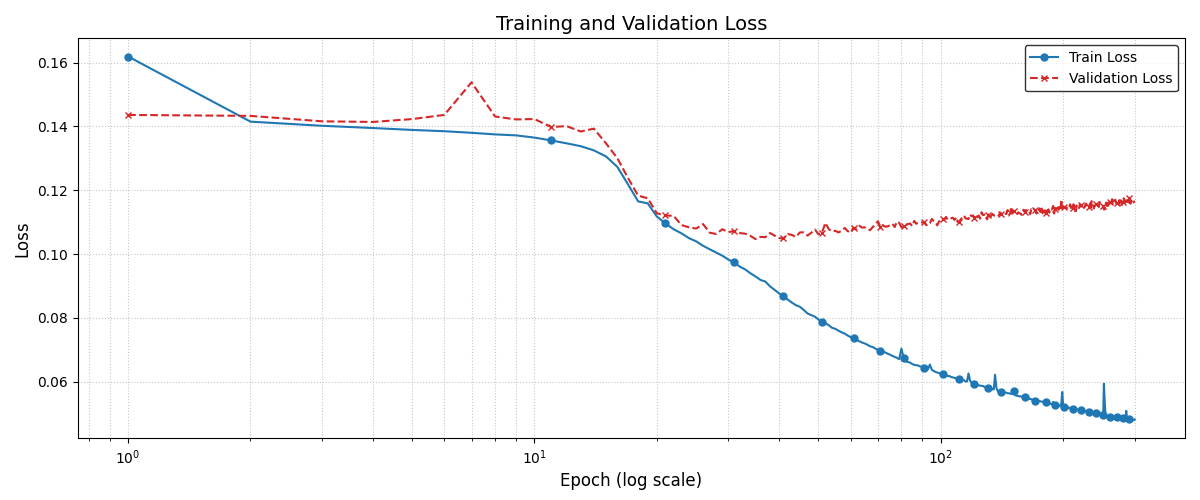
\includegraphics[width=0.7\linewidth]{images/colab_loss_curve.png}
    \newline
    \small Loss curve 
    \newline
    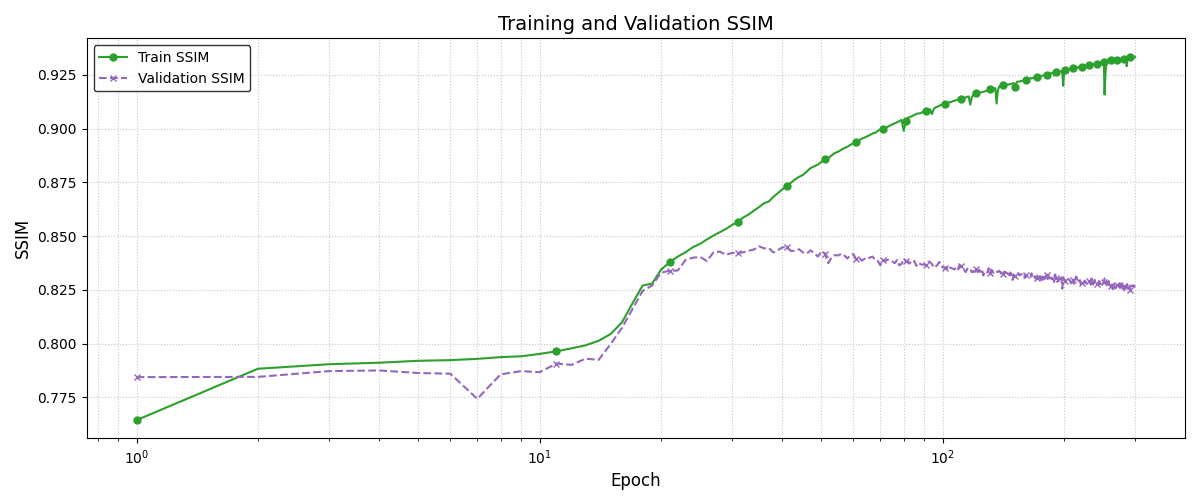
\includegraphics[width=0.7\linewidth]{images/colab_ssim_curve.png}
    \newline
    \small SSIM curve 
\end{frame}

\begin{frame}{Colab Training - Vectorial data vs Directional data}
    \begin{columns}
        \column{0.5\textwidth}
            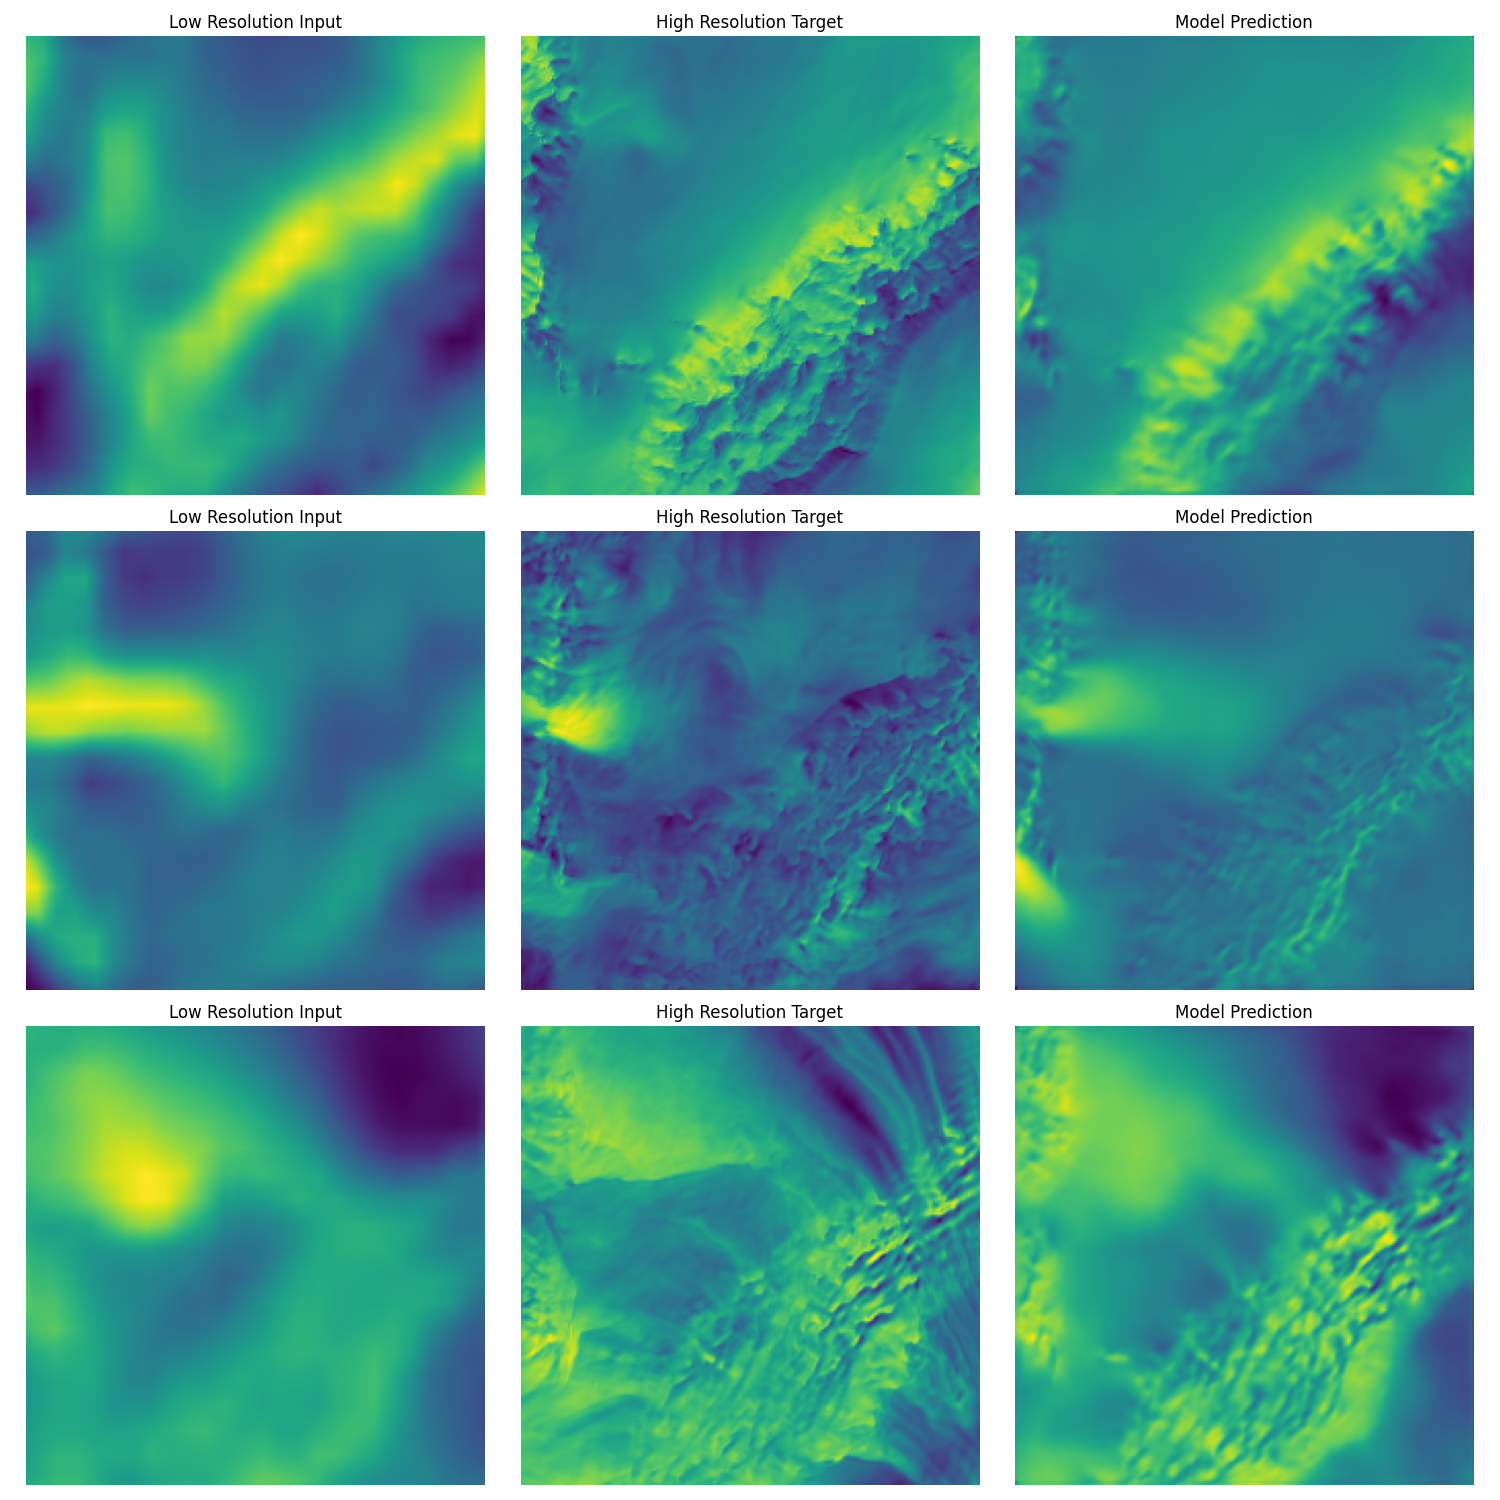
\includegraphics[width=\linewidth]{images/colab_vector_unet_L1SSIM_loss_300_epochs_8_batch_1em3_lr_1em5_weightdecay_best.pt.png}
            \newline
            \centering \small Vector data. SSIM: \texttt{0.84483}
        \column{0.5\textwidth}
            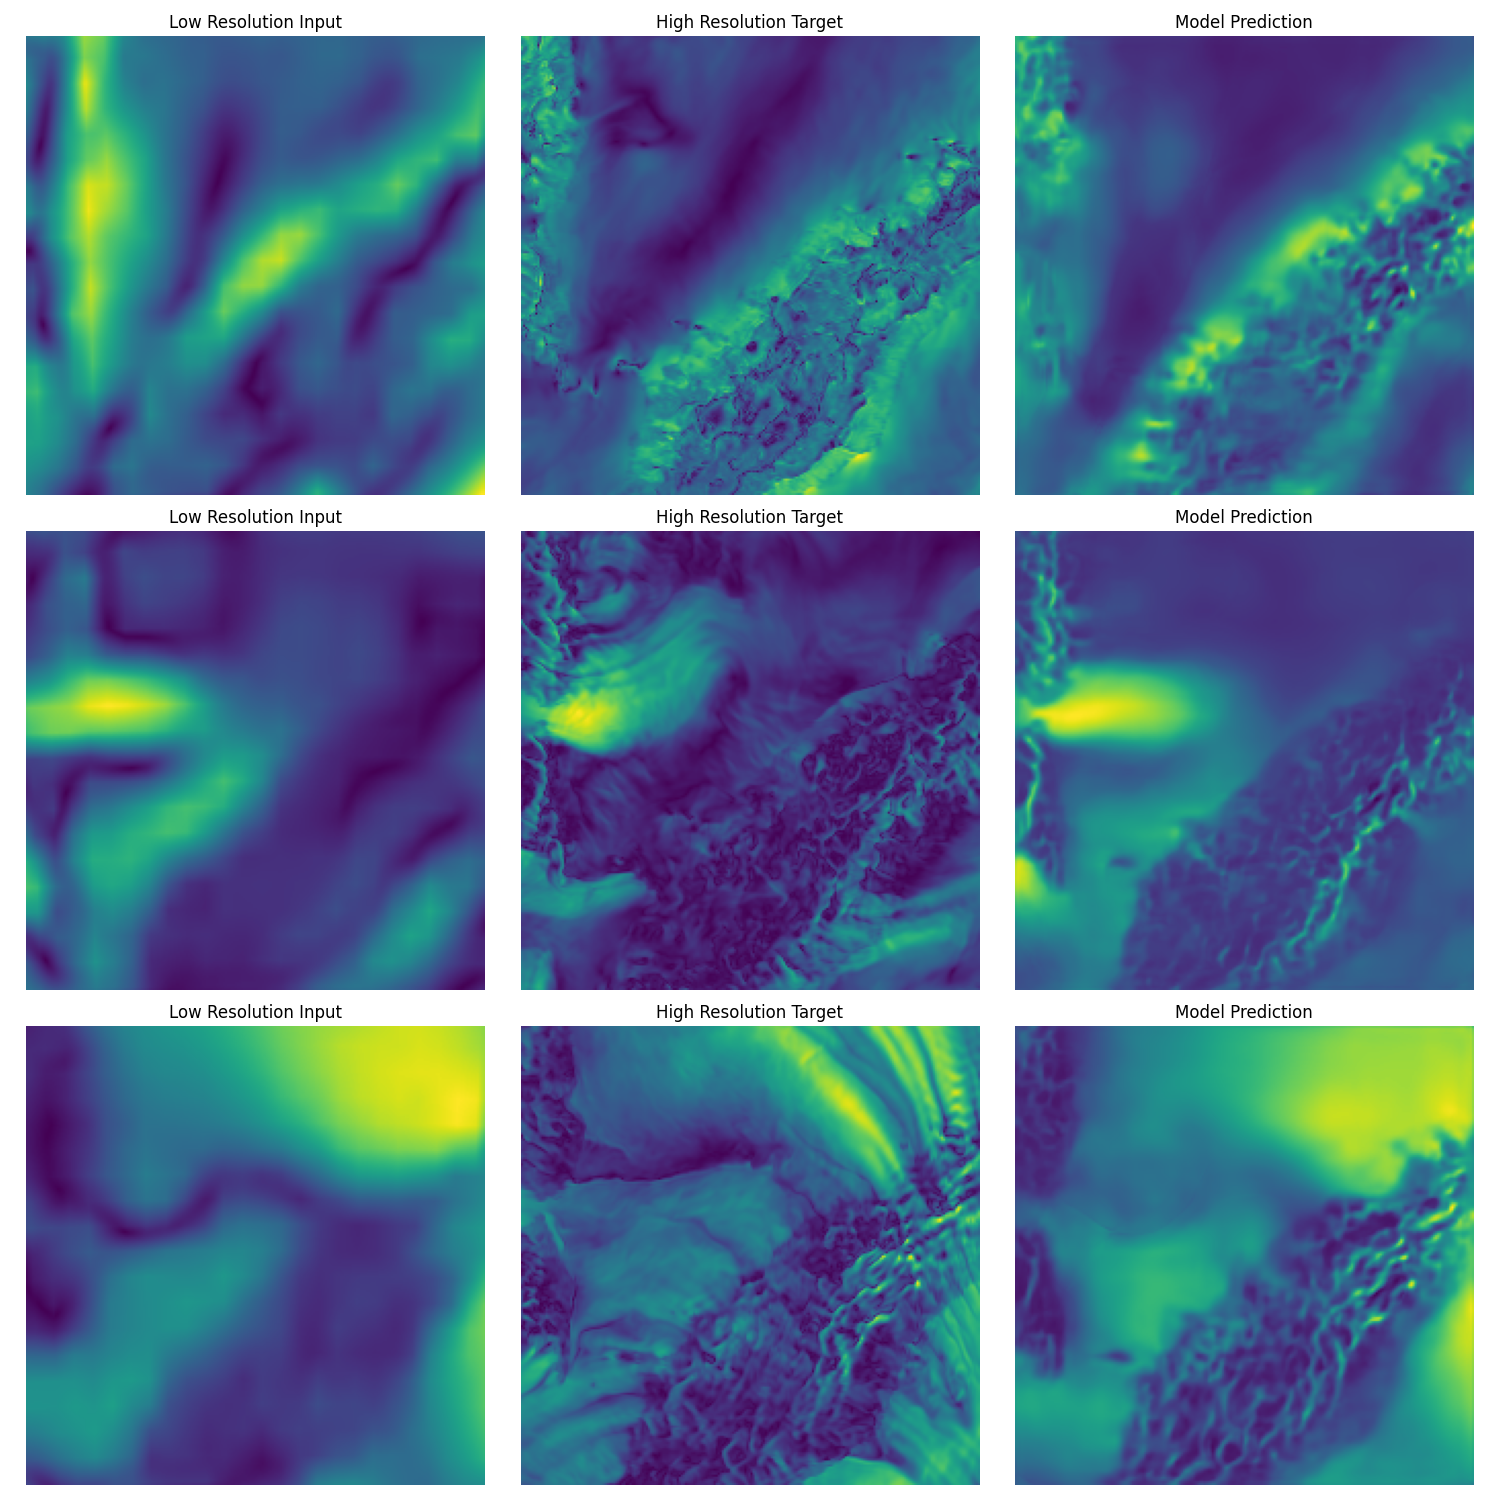
\includegraphics[width=\linewidth]{images/colab_direction_unet_L1SSIM_loss_150_epochs_4_batch_1em3_lr_1em5_weightdecay_best.pt.png}
            \newline
            \centering \small Direction data. SSIM: \texttt{0.48154}
    \end{columns}
\end{frame}

% FEDE
\begin{frame}{Comparison between Vectorial and Directional data}
    \begin{table}[h!]
    \centering
    \begin{tabular}{|l|c|c|}
    \hline
    \textbf{Dataset} & \textbf{Test Loss} & \textbf{Test SSIM} \\
    \hline
    Local Vectors & \underline{0.16610} & \underline{0.75830} \\
    Local Direction & 0.49120 & 0.38960 \\
    Colab Vectors & \textbf{0.10470} & \textbf{0.84535} \\
    Colab Direction & 0.42873 & 0.48154 \\
    \hline
    \end{tabular}
    \caption{Comparison of test loss and SSIM between vectorial and directional data}
    \label{tab:test_results}
    \end{table}
    Directional data underperformed vs. vector-based representations
\end{frame}

% MARZIA
% Section 7: Final Considerations
\section{Final Considerations}
\begin{frame}{Final Considerations}
\justifying
    \textbf{Societal Impact}
    \\More accurate high-resolution forecasts support \textit{agricultural management}, \textit{climate disaster preparedness} and \textit{the coastal/tourist community}.\\\vspace{0.5cm}
    \textbf{Next steps}
    \begin{itemize}
    \justifying
        \item[-] Check whether the \textit{L1 + SSIM} loss still favors accurate reconstruction in complex areas with clear structures, compared to flatter regions where features are harder to predict.
        \item[-] If not, consider analyzing the alpha weight in the loss function to see if the balance between L1 and SSIM is skewed, causing the network to rely too heavily on one component.
    \end{itemize}
\end{frame}
% come ci aspettavamo la rappresentazione con vettori e' quella migliore e quella con intensita' e direzione fa schifo al cazzo

\begin{frame}
    \frametitle{References}
    \printbibliography
\end{frame}
\end{document}

